\documentclass[12pt,letterpaper]{article}
\usepackage{fullpage}
\usepackage[top=2cm, bottom=4.5cm, left=2.5cm, right=2.5cm]{geometry}
\usepackage{amsmath,amsthm,amsfonts,amssymb,amscd}
\usepackage{lastpage}
\usepackage{enumerate}
\usepackage{fancyhdr}
\usepackage{mathrsfs}
\usepackage{xcolor}
\usepackage{graphicx}
\usepackage{listings}
\usepackage{hyperref}
\usepackage{mathtools}
\usepackage{xfrac}
\usepackage{pdfpages}
\usepackage{float} 
\usepackage{subfigure} 

\hypersetup{%
  colorlinks=true,
  linkcolor=blue,
  linkbordercolor={0 0 1}
}
\linespread{1.1}
 
\renewcommand\lstlistingname{Algorithm}
\renewcommand\lstlistlistingname{Algorithms}
\def\lstlistingautorefname{Alg.}

\lstdefinestyle{Python}{
    language        = Python,
    frame           = lines, 
    basicstyle      = \footnotesize,
    keywordstyle    = \color{blue},
    stringstyle     = \color{green},
    commentstyle    = \color{red}\ttfamily
}

\setlength{\parindent}{0.0in}
\setlength{\parskip}{0.05in}

% Edit these as appropriate
\newcommand\course{ConvexOptimization}
\newcommand\hwnumber{6}                  % <-- homework number
\newcommand\NetIDa{SUN Yilin}           % <-- NetID of person #1
\newcommand\NetIDb{520030910361}           % <-- NetID of person #2 (Comment this line out for problem sets)

\pagestyle{fancyplain}
\headheight 35pt
\lhead{\NetIDa}
\lhead{\NetIDa\\\NetIDb}                 % <-- Comment this line out for problem sets (make sure you are person #1)
\chead{\textbf{\Large Homework \hwnumber}}
\rhead{\course \\ \today}
\lfoot{}
\cfoot{}
\rfoot{\small\thepage}
\headsep 1.5em

\begin{document}

\section{}
\subsection*{(a)}
It is $max\{\gamma,1\}$.\\
We know $\nabla f(\boldsymbol{x})=\boldsymbol{Qx}$, where $\boldsymbol{Q}$ is positive definite. So for any $L$ such that $f$ is $L$-smooth, $L$ must satisfy that $||\nabla f(\boldsymbol{x})-\nabla f(\boldsymbol{y})||=||\boldsymbol{Q}(\boldsymbol{x}-\boldsymbol{y})||\leq L(\boldsymbol{x}-\boldsymbol{y})$. Let $(\boldsymbol{x}-\boldsymbol{y})=(d_1,d_2)$, the inequality is equivalent to $\gamma^2d_1^2+d_2^2\leq L^2(d_1^2+d_2^2)$, or $(\gamma^2-L^2)d_1^2+(1-L^2)d_2^2\leq 0$. Since this must hold for any $(d_1,d_2)$, $\gamma^2-L^2\leq0,1-L^2\leq0$. So the smallest $L$ is $max\{\gamma,1\}$.
\subsection*{(b)}
It is $min\{\gamma,1\}$.\\
For any $m$ such that $f$ is $m$-strongly convex, $m$ must satisfy that $f(\boldsymbol{x})-\frac{m}{2}||\boldsymbol{x}||^2$ is convex, that is, $\frac{1}{2}\boldsymbol{x}^T(\boldsymbol{Q}-m\boldsymbol{I})\boldsymbol{x}$ is convex. So $\boldsymbol{Q}-m\boldsymbol{I}$ must be positive semidefinite. So its eigenvalues $\gamma-m$ and $1-m$ must be nonnegative. So the largest $m$ is $min\{\gamma,1\}$.
\subsection*{(c)}
Below are the figures of 2D trajectory of $\boldsymbol{x}_k$ and function values $f(\boldsymbol{x}_k)$. Note that the suboptimality gap $f(\boldsymbol{x}_k)-f(\boldsymbol{x}^*)$ is simply $f(\boldsymbol{x}_k)$ since $f(\boldsymbol{x}^*)=0$.\\
As for convergence, I notice that when stepsize=2.2, it does not converge (I run 20 iterations), while the other three stepsizes all converge. When it does converge, the iterations it takes are as follows (results are from running q1.py):\\
\begin{table}[h]
    \centering
    \begin{tabular}{c|c}
         Stepsize&Iterations  \\\hline
         1&88\\
         0.1&917\\
         0.01&9206
    \end{tabular}
    \caption{Number of Iterations for each stepsize}
    \label{Iters}
\end{table}

\begin{figure}[H]
\centering
\subfigure[stepsize=0.01]{
\label{tr.sub.1}
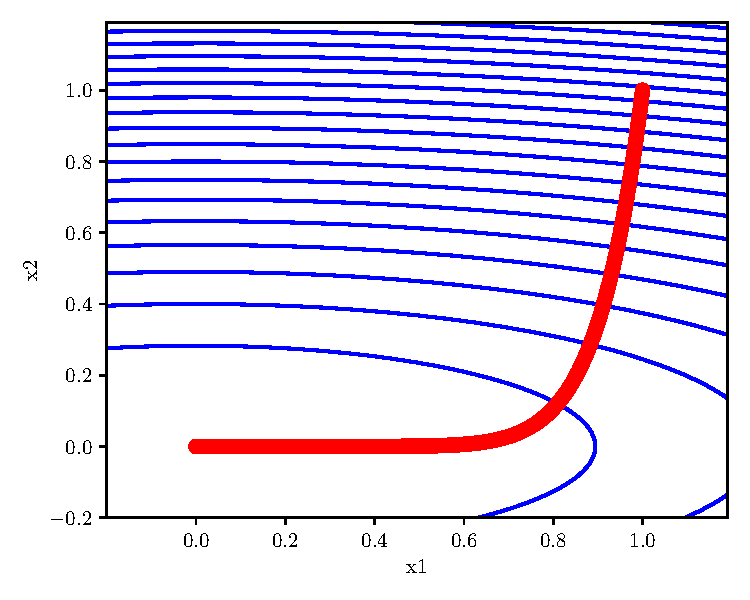
\includegraphics[width=0.45\textwidth]{gd_traces_gamma0.1_ss0.01.pdf}}
\subfigure[stepsize=0.1]{
\label{tr.sub.2}
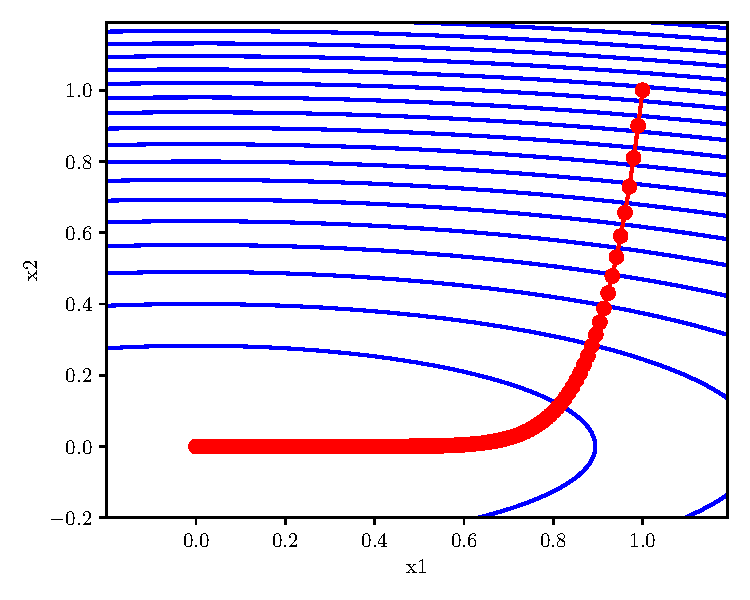
\includegraphics[width=0.45\textwidth]{gd_traces_gamma0.1_ss0.1.pdf}}
\subfigure[stepsize=1]{
\label{tr.sub.3}
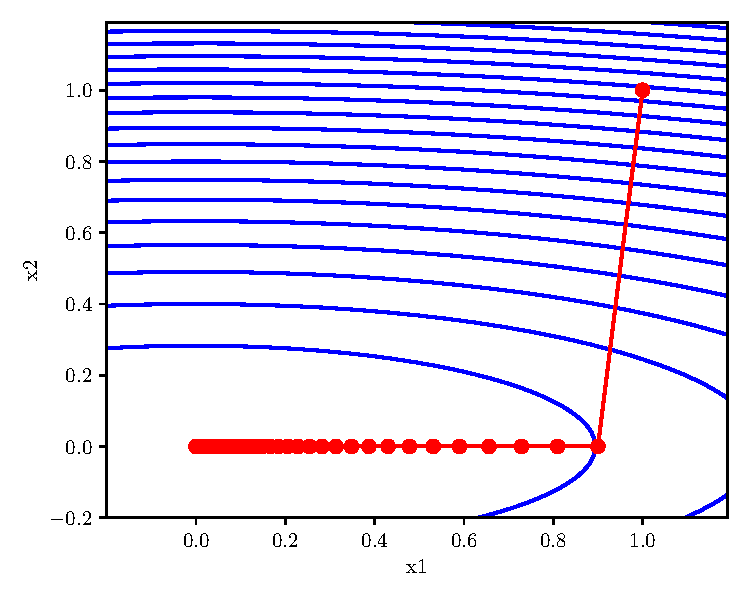
\includegraphics[width=0.45\textwidth]{gd_traces_gamma0.1_ss1.pdf}}
\subfigure[stepsize=2.2]{
\label{tr.sub.4}
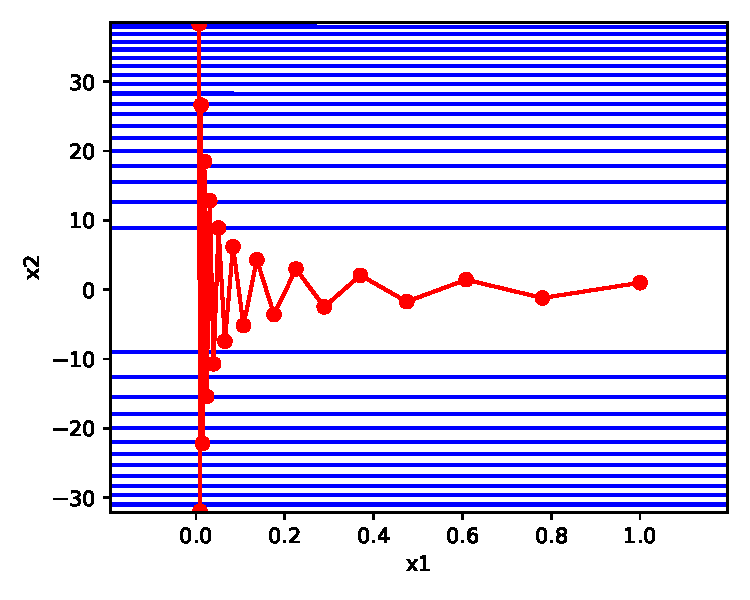
\includegraphics[width=0.45\textwidth]{gd_traces_gamma0.1_ss2.2.pdf}}
\caption{2D trajectory of $\boldsymbol{x}_k$ ($\gamma=0.1$)}
\label{tr}
\end{figure}
From the figure of trajectory(above) we can actually see when stepsize=2.2, $x_1$ goes to $0$ as we descend according to the direction of negative gradient, but $x_2$ oscillates as $x_1$ goes to $0$, it does not converge.\\
From the figure of function value(below) we can see that when stepsize=1, the gradient method actually works well, we do not need a smaller stepsize. Because stepsize=1 only takes less than 100 iterations to get a same outcome as stepsize=0.1 or 0.01, which requires much more iterations.
\begin{figure}[H]
\centering
\subfigure[stepsize=0.01]{
\label{F.sub.1}
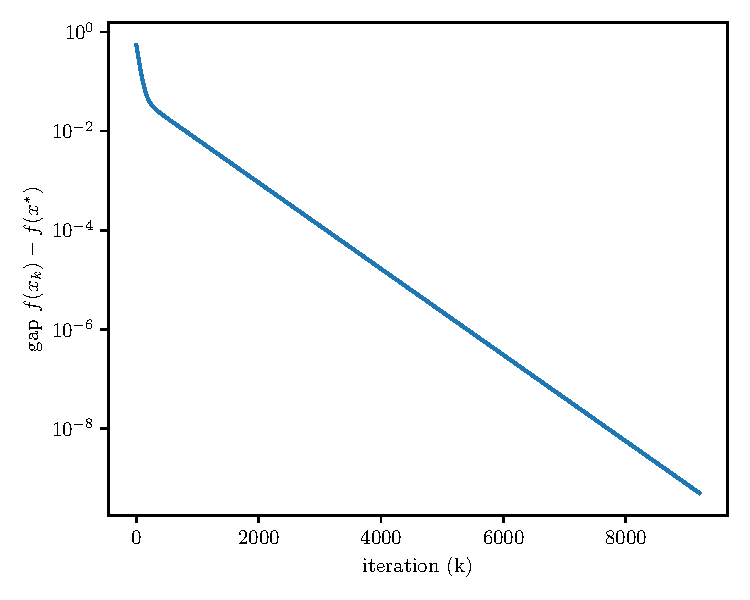
\includegraphics[width=0.45\textwidth]{gd_f_gamma0.1_ss0.01.pdf}}
\subfigure[stepsize=0.1]{
\label{F.sub.2}
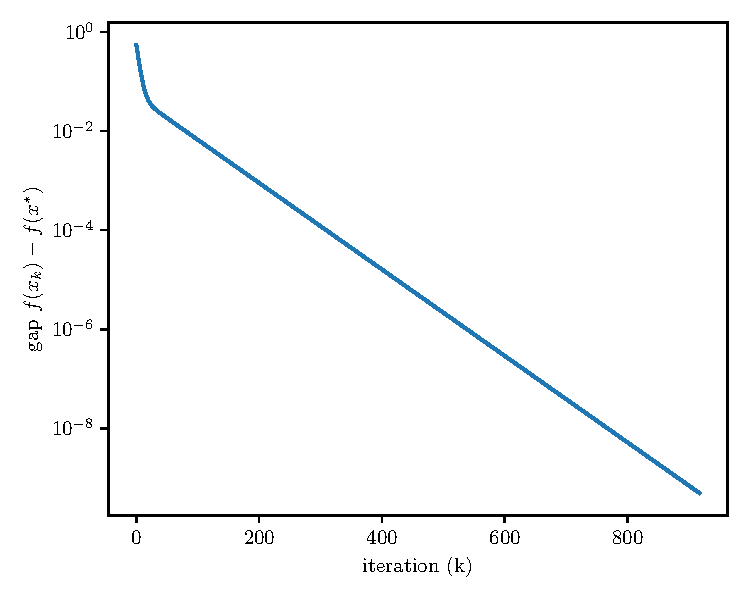
\includegraphics[width=0.45\textwidth]{gd_f_gamma0.1_ss0.1.pdf}}
\subfigure[stepsize=1]{
\label{F.sub.3}
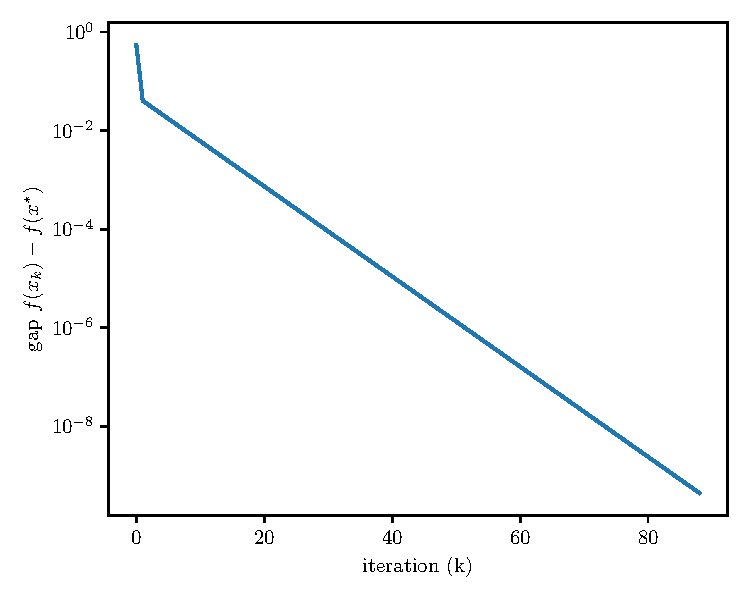
\includegraphics[width=0.45\textwidth]{gd_f_gamma0.1_ss1.pdf}}
\subfigure[stepsize=2.2]{
\label{F.sub.4}
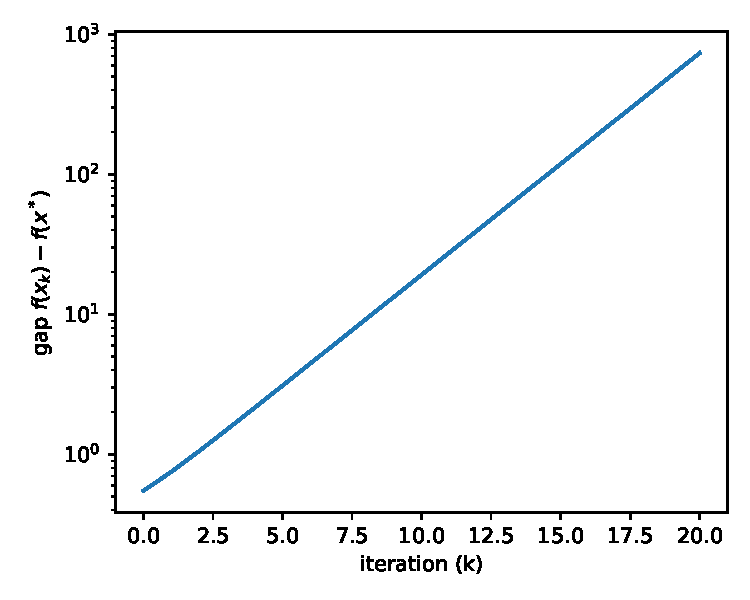
\includegraphics[width=0.45\textwidth]{gd_f_gamma0.1_ss2.2.pdf}}
\caption{Function Values ($\gamma=0.1$)}
\label{function value}
\end{figure}

\subsection*{(d)}
\begin{table}[h]
    \centering
    \begin{tabular}{c|c}
         Gamma&Iterations  \\\hline
         1&1\\
         0.1&88\\
         0.01&688\\
         0.001&4603
    \end{tabular}
    \caption{Number of Iterations for different gamma}
    \label{various gamma}
\end{table}
From the table we can see that as $\gamma$ decreases, the number of iterations increases. And the relation is approximately inversely proportional. The intuition is that the condition number of $\boldsymbol{Q}$ is $\frac{1}{\gamma}$ since $\gamma\leq1$.  So with a larger $\gamma$ we need more iterations to get a same optimum if we are applying the same stepsize.
\section{}
Codes for this problem are in file p2.py. \\
I notice that for a large stepsize it will not converge, for example 3. I choose stepsize=0.01 with a starting point $(1,1)$and the number of iterations is 605. \\
\begin{figure}[H]
\centering
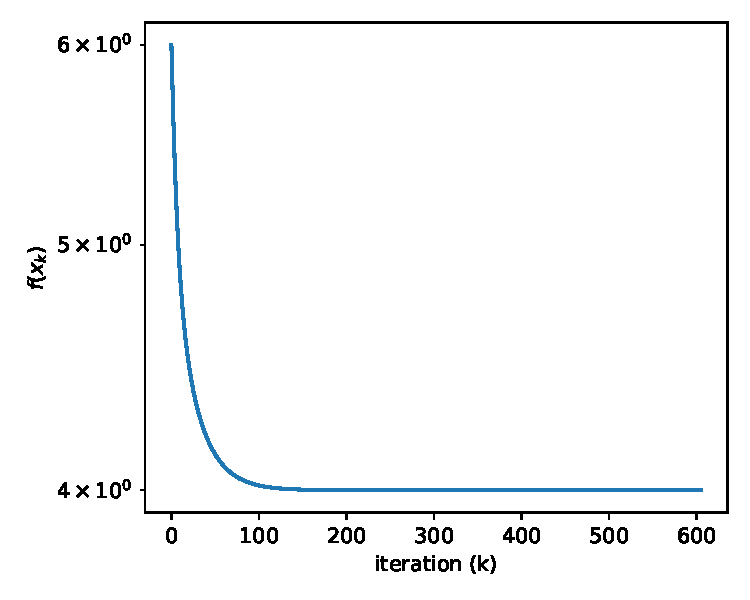
\includegraphics[width=0.45\textwidth]{lso_ss0.01.pdf}
\caption{Least Squares gd with stepsize=0.01 }
\label{lso}
\end{figure}
The solution of closed form in HW5, running gradient descent and using np.linalg.solve are the same. The optimal variables are all $(w_1,w_2)=(1.5,2)$ and the optimal value are all $4$. Figure 3 shows the how the function value descends as we do iterations.
\section{}
The optimal $\boldsymbol{w}^*$ given by running p3.py is (-1.47020052, 4.44377575, -4.37548225). The accuracy is 0.8667. And the classification result is given in the figure below.
\begin{figure}[H]
\centering
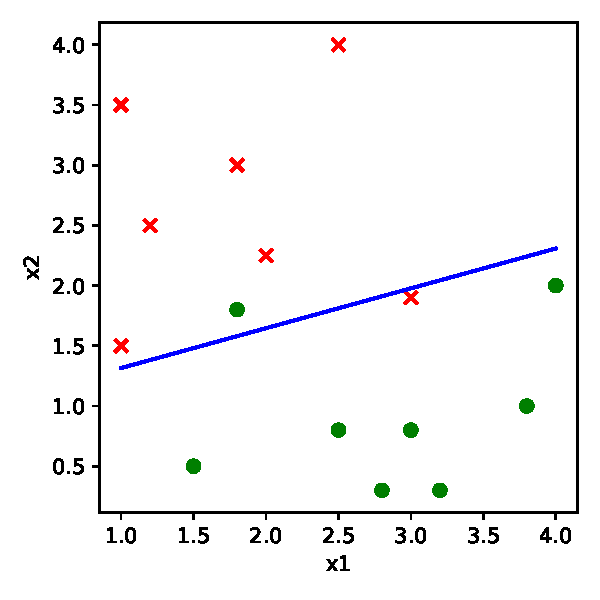
\includegraphics[width=0.45\textwidth]{p3.pdf}
\caption{Classification Result }
\label{logistic}
\end{figure}
\section{}
From $f$ is differentiable and $\alpha$-strongly convex we know $f(\boldsymbol{x})-\frac{\alpha}{2}||\boldsymbol{x}||^2$ is convex. By the first order condition for convexity we get $$f(\boldsymbol{y})-\frac{\alpha}{2}||\boldsymbol{y}||^2-f(\boldsymbol{x})+\frac{\alpha}{2}||\boldsymbol{x}||^2\geq(\nabla f(\boldsymbol{x})-\alpha\boldsymbol{x})^T(\boldsymbol{y}-\boldsymbol{x}), \forall \boldsymbol{x},\boldsymbol{y}$$ From $g$ is $\beta$-smooth we know $$g(\boldsymbol{y})-g(\boldsymbol{x})-\nabla g(\boldsymbol{x})^T(\boldsymbol{y}-\boldsymbol{x})\leq \frac{\beta}{2}||\boldsymbol{y}-\boldsymbol{x}||^2,\forall \boldsymbol{x},\boldsymbol{y}$$ Adding these two inequalities together gives us 
$$[f(\boldsymbol{y})-g(\boldsymbol{y})]-[f(\boldsymbol{x})-g(\boldsymbol{x})]-[\nabla f(\boldsymbol{x})-\nabla g(\boldsymbol{x})]^T(\boldsymbol{y}-\boldsymbol{x})\geq$$ $$\frac{\alpha}{2}(||\boldsymbol{y}||^2-||\boldsymbol{x}||^2)-\alpha\boldsymbol{x}^T\boldsymbol{y}+\alpha||\boldsymbol{x}||^2-\frac{\beta}{2}(||\boldsymbol{y}||^2+||\boldsymbol{x}||^2)+\beta\boldsymbol{x}^T\boldsymbol{y},\forall \boldsymbol{x},\boldsymbol{y}$$
RHS is simply $$\frac{\alpha-\beta}{2}||\boldsymbol{y}-
\boldsymbol{x}||^2$$
Which is greater or equal to $0$. So$$[f(\boldsymbol{y})-g(\boldsymbol{y})]\geq[f(\boldsymbol{x})-g(\boldsymbol{x})]+[\nabla f(\boldsymbol{x})-\nabla g(\boldsymbol{x})]^T(\boldsymbol{y}-\boldsymbol{x}),\forall \boldsymbol{x},\boldsymbol{y}$$
Or equivalently$$h(\boldsymbol{y})\geq h(\boldsymbol{x})+\nabla h(\boldsymbol{x})^T(\boldsymbol{y}-\boldsymbol{x}),\forall\boldsymbol{x},\boldsymbol{y}$$
Then by first order condition for convexity we know $h$ is convex.
\end{document}
